\documentclass[tikz,border=8pt]{standalone}
\usepackage{xcolor}
\usetikzlibrary{arrows.meta,positioning,fit,backgrounds}
\begin{document}
% Counterfactual topology
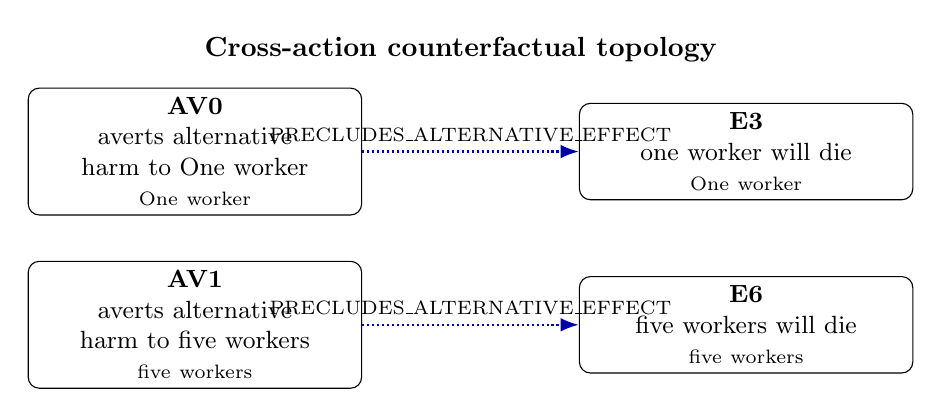
\begin{tikzpicture}[>=Latex,event/.style={draw,rounded corners,align=center,text width=4cm,minimum height=1.2cm,font=\small},counter/.style={->,thick,densely dotted,draw=blue!65!black}]
\node[font=\bfseries,anchor=west] at (0,1.3) {Cross-action counterfactual topology};
\node[event] (eAV0) at (0,0.0) {\textbf{AV0}\\averts alternative harm to One worker\\\scriptsize One worker};
\node[event] (eE3) at (7,0.0) {\textbf{E3}\\one worker will die\\\scriptsize One worker};
\node[event] (eAV1) at (0,-2.2) {\textbf{AV1}\\averts alternative harm to five workers\\\scriptsize five workers};
\node[event] (eE6) at (7,-2.2) {\textbf{E6}\\five workers will die\\\scriptsize five workers};
\draw[counter] (eAV0) -- node[above,font=\scriptsize] {PRECLUDES\_ALTERNATIVE\_EFFECT} (eE3);
\draw[counter] (eAV1) -- node[above,font=\scriptsize] {PRECLUDES\_ALTERNATIVE\_EFFECT} (eE6);
\end{tikzpicture}
\end{document}
